The logarithm terms are integrated in much the same way they were in the first mandatory assignment.
The boundary element method assumes the potential is constant, set to the value of the midpoint between nodes.
Integration of the logarithm terms in the \textsc{Green} function is outlined in the lecture notes from January 28\textsuperscript{st}.
The gradient of the other terms are given to be
\[
    \deex\green = \kappa \big( \Im{(f_1)} + i \Im{(f_2)} \big),
\]\[
    \deey\green = \kappa \big( \Re{(f_1)} + i\Re{(f_2)} \big),
\]
and are treated with a midtpoint rule, setting the complex variable
\[
    \ezh = \kappa\big(\che_m  + \che_n - i (\zhe_m  - \zhe_n) \big).
\]
The boundary we discretize with a \textsc{Chebyshov} distribution in two coordinates $\xtt_\mathtt{p}$ and $\xtt_\mathtt{m}$.
Constructing a partition of the interval whose midpoints forms \textsc{Chebyshov} distribution seems to be more effort than it is worth, so we concede that \textsc{Chebyshov} distributions in $\xtt_{\mathtt{p}}$ and $\xtt_{\mathtt{m}}$ suffice to get accurate enough results near the corners of the box.
\begin{Figure}
    \centering
    \captionsetup{type = figure}
    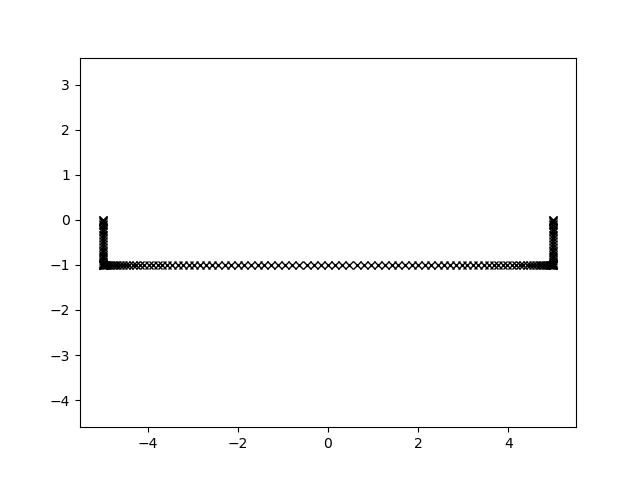
\includegraphics[width = \textwidth]{box_L10.png}
    \caption{Rectangle with $\sfrac{L}{D} = 10$}
\end{Figure}
